\documentclass[11pt,a4paper,twoside]{report}

% ============================================================================
% PACKAGES
% ============================================================================

% Encoding and fonts
\usepackage[utf8]{inputenc}
\usepackage[T1]{fontenc}
\usepackage{lmodern}
\usepackage{microtype}

% Page layout
\usepackage[
    top=2.5cm,
    bottom=2.5cm,
    left=3cm,
    right=2.5cm,
    headheight=14pt
]{geometry}

% Colors
\usepackage[dvipsnames,svgnames,table]{xcolor}
\definecolor{primaryblue}{RGB}{37, 99, 235}
\definecolor{secondarygreen}{RGB}{34, 197, 94}
\definecolor{warningamber}{RGB}{245, 158, 11}
\definecolor{dangerred}{RGB}{239, 68, 68}
\definecolor{codebg}{RGB}{248, 250, 252}
\definecolor{codeframe}{RGB}{226, 232, 240}
\definecolor{linkblue}{RGB}{59, 130, 246}

% Graphics and diagrams
\usepackage{tikz}
\usetikzlibrary{
    shapes.geometric,
    shapes.symbols,
    shapes.misc,
    shapes.arrows,
    arrows.meta,
    positioning,
    calc,
    fit,
    backgrounds,
    decorations.pathreplacing,
    patterns,
    shadows.blur
}

% Tables
\usepackage{booktabs}
\usepackage{tabularx}
\usepackage{longtable}
\usepackage{multirow}
\usepackage{array}

% Lists
\usepackage{enumitem}
\setlist{noitemsep,topsep=0pt}

% Code listings
\usepackage{listings}
\usepackage{fancyvrb}

\lstdefinestyle{code}{
    backgroundcolor=\color{codebg},
    basicstyle=\ttfamily\small,
    breakatwhitespace=false,
    breaklines=true,
    captionpos=b,
    commentstyle=\color{gray},
    frame=single,
    rulecolor=\color{codeframe},
    keepspaces=true,
    keywordstyle=\color{primaryblue}\bfseries,
    numbers=left,
    numbersep=8pt,
    numberstyle=\tiny\color{gray},
    showspaces=false,
    showstringspaces=false,
    showtabs=false,
    stringstyle=\color{secondarygreen},
    tabsize=2,
    xleftmargin=1em,
    framexleftmargin=1em
}

\lstdefinestyle{yaml}{
    style=code,
    language=yaml,
    morekeywords={route_generation,method,num_routes,gemini,image_model,text_model,analysis_model}
}

\lstdefinestyle{python}{
    style=code,
    language=Python,
    morekeywords={class,def,async,await,BaseModel,Literal,Optional,float,int,str,bool,list}
}

\lstdefinestyle{typescript}{
    style=code,
    language=Java,
    morekeywords={interface,type,const,let,async,await,function,string,number,boolean}
}

\lstdefinestyle{json}{
    style=code,
    stringstyle=\color{dangerred},
    morestring=[b]"
}

\lstdefinestyle{bash}{
    style=code,
    language=bash,
    morekeywords={docker,compose,git,curl,npm,gcloud}
}

\lstset{style=code}

% Hyperlinks
\usepackage[
    colorlinks=true,
    linkcolor=primaryblue,
    urlcolor=linkblue,
    citecolor=primaryblue,
    bookmarks=true,
    bookmarksnumbered=true,
    pdfstartview=FitH
]{hyperref}

% Headers and footers
\usepackage{fancyhdr}
\pagestyle{fancy}
\fancyhf{}
\fancyhead[LE,RO]{\thepage}
\fancyhead[LO]{\nouppercase{\rightmark}}
\fancyhead[RE]{\nouppercase{\leftmark}}
\renewcommand{\headrulewidth}{0.4pt}

% Chapter styling
\usepackage{titlesec}
\titleformat{\chapter}[display]
    {\normalfont\huge\bfseries\color{primaryblue}}
    {\chaptertitlename\ \thechapter}
    {20pt}
    {\Huge}
\titlespacing*{\chapter}{0pt}{-20pt}{40pt}

% Section styling
\titleformat{\section}
    {\normalfont\Large\bfseries\color{primaryblue}}
    {\thesection}
    {1em}
    {}

\titleformat{\subsection}
    {\normalfont\large\bfseries}
    {\thesubsection}
    {1em}
    {}

% Boxes for notes and warnings
\usepackage[most]{tcolorbox}

\newtcolorbox{notebox}{
    colback=blue!5!white,
    colframe=primaryblue,
    fonttitle=\bfseries,
    title=Note,
    boxrule=0.5pt,
    arc=2pt,
    left=6pt,
    right=6pt,
    top=6pt,
    bottom=6pt
}

\newtcolorbox{warningbox}{
    colback=yellow!10!white,
    colframe=warningamber,
    fonttitle=\bfseries,
    title=Warning,
    boxrule=0.5pt,
    arc=2pt,
    left=6pt,
    right=6pt,
    top=6pt,
    bottom=6pt
}

\newtcolorbox{tipbox}{
    colback=green!5!white,
    colframe=secondarygreen,
    fonttitle=\bfseries,
    title=Tip,
    boxrule=0.5pt,
    arc=2pt,
    left=6pt,
    right=6pt,
    top=6pt,
    bottom=6pt
}

% Glossary
\usepackage[acronym,toc]{glossaries}
\makeglossaries

% Bibliography (if needed)
\usepackage[style=numeric,sorting=none]{biblatex}

% Math (for any formulas)
\usepackage{amsmath}
\usepackage{amssymb}

% Misc
\usepackage{lipsum}
\usepackage{graphicx}
\usepackage{float}
\usepackage{caption}
\usepackage{subcaption}

% ============================================================================
% TIKZ STYLES
% ============================================================================

\tikzstyle{component} = [
    rectangle,
    rounded corners=3pt,
    draw=codeframe,
    fill=codebg,
    text centered,
    minimum height=1cm,
    minimum width=2.5cm,
    font=\small
]

\tikzstyle{service} = [
    rectangle,
    rounded corners=3pt,
    draw=primaryblue,
    fill=primaryblue!10,
    text centered,
    minimum height=1cm,
    minimum width=2.5cm,
    font=\small\bfseries
]

\tikzstyle{external} = [
    rectangle,
    rounded corners=3pt,
    draw=secondarygreen,
    fill=secondarygreen!10,
    text centered,
    minimum height=1cm,
    minimum width=2.5cm,
    font=\small
]

\tikzstyle{process} = [
    rectangle,
    draw=gray,
    fill=white,
    text centered,
    minimum height=0.8cm,
    minimum width=3cm,
    font=\small
]

\tikzstyle{arrow} = [
    ->,
    >=Stealth,
    thick
]

\tikzstyle{dashedarrow} = [
    ->,
    >=Stealth,
    dashed
]

\tikzstyle{container} = [
    rectangle,
    rounded corners=5pt,
    draw=gray!50,
    dashed,
    inner sep=10pt
]

% ============================================================================
% DOCUMENT INFO
% ============================================================================

\title{
    \vspace{-1cm}
    {\Huge\bfseries\color{primaryblue} GeoRoute}\\[0.5cm]
    {\LARGE Project Manual}\\[1cm]
    {\large AI-Powered Tactical Route Planning System}
}

\author{
    \textbf{Version 1.0}\\[0.5cm]
    Technical Documentation
}

\date{February 2026}

% ============================================================================
% DOCUMENT
% ============================================================================

\begin{document}

% Title page
\begin{titlepage}
    \centering
    \vspace*{2cm}

    {\Huge\bfseries\color{primaryblue} GeoRoute\par}
    \vspace{1cm}
    {\LARGE Project Manual\par}
    \vspace{0.5cm}
    {\large AI-Powered Tactical Route Planning System\par}

    \vspace{2cm}

    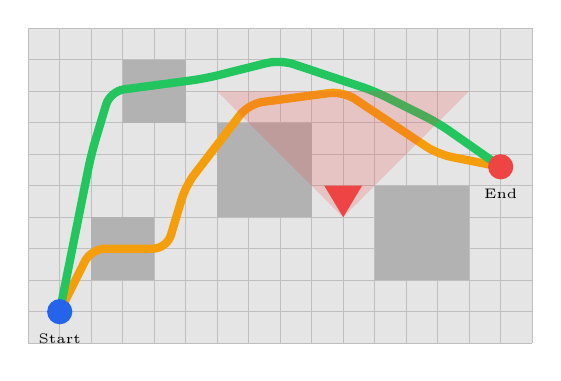
\begin{tikzpicture}[scale=0.8]
        % Satellite image representation
        \fill[gray!20] (0,0) rectangle (8,5);
        \draw[gray!50] (0,0) grid[step=0.5] (8,5);

        % Buildings
        \fill[gray!60] (1,1) rectangle (2,2);
        \fill[gray!60] (3,2) rectangle (4.5,3.5);
        \fill[gray!60] (5.5,1) rectangle (7,2.5);
        \fill[gray!60] (1.5,3.5) rectangle (2.5,4.5);

        % Route (orange - balanced)
        \draw[warningamber, line width=3pt, rounded corners=5pt]
            (0.5,0.5) -- (1,1.5) -- (2.2,1.5) -- (2.5,2.5) -- (3.5,3.8) -- (5,4) -- (6.5,3) -- (7.5,2.8);

        % Route (green - stealth)
        \draw[secondarygreen, line width=3pt, rounded corners=5pt]
            (0.5,0.5) -- (0.8,2) -- (1,3) -- (1.3,4) -- (2.8,4.2) -- (4,4.5) -- (5.5,4) -- (6.5,3.5) -- (7.5,2.8);

        % Start point
        \fill[primaryblue] (0.5,0.5) circle (0.2);
        \node[below, font=\tiny] at (0.5,0.3) {Start};

        % End point
        \fill[dangerred] (7.5,2.8) circle (0.2);
        \node[below, font=\tiny] at (7.5,2.6) {End};

        % Enemy
        \fill[dangerred] (5,2) -- (5.3,2.5) -- (4.7,2.5) -- cycle;

        % Vision cone
        \fill[dangerred, opacity=0.2] (5,2) -- (3,4) -- (7,4) -- cycle;
    \end{tikzpicture}

    \vspace{2cm}

    {\large\bfseries Version 1.0\par}
    \vspace{0.5cm}
    {\large February 2026\par}

    \vfill

    {\small Technical Documentation for System Administrators, Tactical Analysts, and Developers\par}
\end{titlepage}

% Table of contents
\tableofcontents
\newpage

% ============================================================================
% EXECUTIVE SUMMARY
% ============================================================================

\chapter*{Executive Summary}
\addcontentsline{toc}{chapter}{Executive Summary}

GeoRoute represents a significant advancement in tactical route planning technology, combining the analytical power of Google's latest Gemini AI models with real-world satellite imagery to provide military planners and tactical analysts with an intelligent decision-support system. The platform addresses a fundamental challenge in tactical operations: the need to quickly assess and plan infantry movement routes while accounting for terrain, enemy positions, cover availability, and approach angles.

Traditional route planning relies heavily on manual map analysis and the experience of individual planners. GeoRoute augments this process by automatically analyzing satellite imagery, identifying potential cover positions, calculating exposure to enemy observation, and generating optimized tactical routes with quantified risk assessments. The system does not replace human judgment but rather provides planners with comprehensive, data-driven analysis to inform their decisions.

This manual serves as the definitive reference for deploying, configuring, operating, and extending the GeoRoute system. It is intended for:
\begin{itemize}
    \item \textbf{System Administrators} responsible for installation and maintenance
    \item \textbf{Tactical Analysts} who will use the system operationally
    \item \textbf{Developers} who may need to customize or extend its capabilities
\end{itemize}

% ============================================================================
% WHAT'S NEW IN VERSION 2.0
% ============================================================================

\chapter*{What's New in Version 2.0}
\addcontentsline{toc}{chapter}{What's New in Version 2.0}

Version 2.0 introduces significant infrastructure improvements for production deployments:

\section*{NGINX Reverse Proxy}
\begin{itemize}
    \item All traffic now routes through NGINX on port 80
    \item Rate limiting protects against abuse (10 req/s API, 30 req/s general)
    \item Gzip compression reduces bandwidth usage
    \item Security headers prevent common web vulnerabilities
    \item Long timeouts (3 minutes) for AI operations
    \item SSE (Server-Sent Events) properly proxied for progress streaming
\end{itemize}

\section*{Vertex AI Support}
\begin{itemize}
    \item Production-recommended AI backend with higher quotas
    \item Service account authentication for enterprise deployments
    \item Better reliability and faster response times
    \item Seamless fallback to AI Studio for development
\end{itemize}

\section*{Load Balancing}
\begin{itemize}
    \item Scale backend replicas with single command: \texttt{docker compose up -d --scale georoute-backend=3}
    \item NGINX IP hash algorithm ensures sticky sessions for SSE progress
    \item Handle more concurrent users during AI processing
\end{itemize}

\section*{Unified Configuration}
\begin{itemize}
    \item Single docker-compose.yml for all environments
    \item Consolidated .env.example with all options
    \item Simplified deployment process
\end{itemize}

\section*{Error Sanitization}
\begin{itemize}
    \item User-friendly error messages without exposing internals
    \item Proper HTTP status codes (429 for rate limits, 503 for unavailable)
    \item Detailed logging for administrators
\end{itemize}

% ============================================================================
% CHAPTER 1: INTRODUCTION
% ============================================================================

\chapter{Introduction}

\section{What is GeoRoute?}

GeoRoute is an AI-powered tactical route planning system designed for infantry movement analysis. At its core, the system leverages Google's Gemini family of large language models, which possess the remarkable ability to understand and analyze visual imagery, to perform sophisticated tactical assessments that would traditionally require significant manual effort and expertise.

The system operates on a fundamental principle: tactical route planning is inherently a visual and spatial problem. By providing AI models with actual satellite imagery of the operational area, along with marked positions of friendly and enemy forces, the system can generate analysis that accounts for real-world terrain features such as buildings, vegetation, roads, and open ground. This approach yields results that are grounded in the actual geography of the area rather than abstract calculations.

GeoRoute integrates four primary technologies to deliver its capabilities:

\subsection{Satellite Imagery Foundation}

The system utilizes ESRI World Imagery, the same high-resolution satellite imagery used by professional GIS applications worldwide. This imagery is fetched in real-time and stitched together to create seamless maps of any area within the supported region. The use of actual satellite imagery, rather than simplified maps, allows the AI to identify terrain features, buildings, roads, and vegetation that affect tactical movement.

\subsection{Advanced AI Analysis}

Google's Gemini 3 Pro model, specifically the image-generation variant, can actually draw on images. When given a satellite image with marked start and end positions, it generates tactical routes by drawing directly on the imagery, creating visually intuitive route overlays that account for obstacles and cover. The Gemini 3 Flash model, optimized for vision analysis, then examines these routes to assess risk, identify weak points, and generate recommendations.

\subsection{Tactical Simulation Engine}

Beyond AI analysis, the system includes a geometric simulation engine that models enemy fields of view as vision cones. These cones are calculated based on realistic parameters for different enemy types (snipers with narrow but long-range vision, riflemen with wider but shorter-range observation). The AI then analyzes which portions of a route fall within these vision cones and, critically, whether terrain features provide concealment.

\subsection{Interactive Mapping Interface}

The user interface is built on Leaflet, an industry-standard mapping library, enhanced with military-specific functionality. Users can place units using NATO APP-6 standard symbology, draw movement routes, position enemies with specific facing directions, and visualize the complete tactical picture on a single integrated display.

\section{Core Capabilities}

The system provides five primary capabilities, each designed to address specific aspects of tactical route planning:

\begin{description}
    \item[AI-Powered Route Generation] allows users to simply mark friendly and enemy positions, after which the AI generates a tactical route. The AI draws a single optimized cyan route directly on the satellite imagery, following streets and paths between buildings while avoiding obstacles.

    \item[User Route Evaluation] enables experienced planners to draw their own proposed routes and submit them for AI analysis. This capability recognizes that human expertise remains essential and provides a way to validate planned routes against AI assessment.

    \item[Tactical Simulation] provides the most detailed analysis by combining geometric vision cone calculations with AI-based cover assessment. The system first calculates which route segments geometrically fall within enemy observation, then uses AI vision analysis to determine whether buildings, walls, or terrain actually block the line of sight.

    \item[Multi-Dimensional Scoring] quantifies tactical quality across four dimensions: stealth, safety, terrain usage, and flanking. These individual scores combine into an overall rating that allows direct comparison between route options.

    \item[Verdict Classification] translates numerical scores into actionable categories: EXCELLENT, GOOD, ACCEPTABLE, or RISKY.
\end{description}

\section{Geographic Scope}

GeoRoute is configured to operate exclusively within the Gulf Cooperation Council (GCC) region, encompassing Saudi Arabia, the United Arab Emirates, Kuwait, Bahrain, Qatar, and Oman. This geographic restriction is defined as the area shown in Table~\ref{tab:gcc-bounds}.

\begin{table}[h]
\centering
\caption{GCC Region Boundaries}
\label{tab:gcc-bounds}
\begin{tabular}{lc}
\toprule
\textbf{Boundary} & \textbf{Coordinate} \\
\midrule
Northern Latitude & 32.0°N \\
Southern Latitude & 12.0°N \\
Eastern Longitude & 60.0°E \\
Western Longitude & 34.0°E \\
\bottomrule
\end{tabular}
\end{table}

% ============================================================================
% CHAPTER 2: INSTALLATION
% ============================================================================

\chapter{Installation}

This chapter provides comprehensive guidance for deploying GeoRoute in various environments, from local development setups to production deployments. The system is containerized using Docker, which ensures consistent behavior across different operating systems and simplifies dependency management.

\section{Prerequisites}

Before beginning installation, ensure your system meets the requirements listed in Table~\ref{tab:prerequisites}.

\begin{table}[h]
\centering
\caption{System Prerequisites}
\label{tab:prerequisites}
\begin{tabular}{lll}
\toprule
\textbf{Requirement} & \textbf{Version} & \textbf{Purpose} \\
\midrule
Docker & 20.10+ & Container runtime \\
Docker Compose & 2.0+ & Multi-container orchestration \\
Google Cloud Account & --- & API access \\
Git & 2.0+ & Clone repository \\
\bottomrule
\end{tabular}
\end{table}

\section{API Keys Required}

GeoRoute requires access to Google Cloud services for both its mapping capabilities and AI analysis. You will need to obtain two types of credentials:

\begin{enumerate}
    \item \textbf{Google Maps API Key} --- for satellite imagery and elevation data
    \item \textbf{AI Service Credentials} --- either:
    \begin{itemize}
        \item Gemini API key (AI Studio) for simple deployments, or
        \item Vertex AI credentials for production use with higher rate limits
    \end{itemize}
\end{enumerate}

\subsection{Google Maps API Key}

\begin{enumerate}
    \item Navigate to \href{https://console.cloud.google.com/apis/credentials}{Google Cloud Console}
    \item Create a new project or select existing
    \item Enable the following APIs:
    \begin{itemize}
        \item Maps Elevation API
        \item Maps Static API
    \end{itemize}
    \item Create an API key with these APIs enabled
\end{enumerate}

\subsection{Gemini API Key (AI Studio)}

\begin{enumerate}
    \item Navigate to \href{https://aistudio.google.com/app/apikey}{AI Studio}
    \item Create a new API key
    \item Key format: \texttt{AIzaSy...} (starts with ``AIzaSy'')
\end{enumerate}

\section{Basic Installation}

\begin{lstlisting}[style=bash]
# Clone the repository
git clone https://github.com/0aub/GeoRoute.git
cd GeoRoute

# Create environment file
cp .env.example .env

# Edit .env with your API keys
nano .env

# Start all services
docker compose up --build

# Or run in background
docker compose up --build -d
\end{lstlisting}

\section{Environment Variables}

Create a \texttt{.env} file with the variables shown in Listing~\ref{lst:env-config}.

\begin{lstlisting}[style=bash,caption={Environment Configuration},label={lst:env-config}]
# Server Configuration
BACKEND_PORT=8001
BACKEND_HOST=0.0.0.0
UI_PORT=8080
CORS_ORIGINS=http://localhost:8080
VITE_API_URL=http://localhost:8001

# Google APIs (Required)
GOOGLE_CLOUD_PROJECT=your-project-id
GOOGLE_MAPS_API_KEY=your-google-maps-api-key

# AI Service - Choose ONE option:
# Option 1: AI Studio
GEMINI_API_KEY=your-gemini-api-key

# Option 2: Vertex AI
# USE_VERTEX_AI=true
# VERTEX_LOCATION=us-central1
\end{lstlisting}

\section{Vertex AI Setup}

For production deployments with higher rate limits, configure Vertex AI:

\begin{enumerate}
    \item \textbf{Create Service Account}
    \begin{lstlisting}[style=bash]
gcloud iam service-accounts create georoute-sa \
  --display-name="GeoRoute Service Account"
    \end{lstlisting}

    \item \textbf{Grant Permissions}
    \begin{lstlisting}[style=bash]
gcloud projects add-iam-policy-binding YOUR_PROJECT_ID \
  --member="serviceAccount:georoute-sa@YOUR_PROJECT_ID.iam.gserviceaccount.com" \
  --role="roles/aiplatform.user"
    \end{lstlisting}

    \item \textbf{Download JSON Key}
    \begin{lstlisting}[style=bash]
gcloud iam service-accounts keys create service-account.json \
  --iam-account=georoute-sa@YOUR_PROJECT_ID.iam.gserviceaccount.com
    \end{lstlisting}

    \item \textbf{Place Key File} in the GeoRoute root directory

    \item \textbf{Configure Environment}
    \begin{lstlisting}[style=bash]
USE_VERTEX_AI=true
VERTEX_LOCATION=us-central1
GOOGLE_CLOUD_PROJECT=your-project-id
    \end{lstlisting}
\end{enumerate}

\section{Running the System}

With configuration complete, start the GeoRoute services using Docker Compose:

\begin{lstlisting}[style=bash]
# Start all services (foreground with logs)
docker compose up --build

# Or run in background (detached mode)
docker compose up --build -d

# View logs when running in background
docker compose logs -f
\end{lstlisting}

The first startup will take several minutes as Docker builds the container images. Subsequent starts are much faster as cached layers are reused.

\section{Accessing the Application}

After successful startup, the services are available at the URLs shown in Table~\ref{tab:service-urls}.

\begin{table}[h]
\centering
\caption{Service URLs}
\label{tab:service-urls}
\begin{tabular}{lll}
\toprule
\textbf{Service} & \textbf{URL} & \textbf{Description} \\
\midrule
UI & \texttt{http://localhost:8080} & Main application interface \\
API & \texttt{http://localhost:8001} & Backend REST API \\
Health & \texttt{http://localhost:8001/api/health} & Health check endpoint \\
\bottomrule
\end{tabular}
\end{table}

\section{Stopping the System}

To gracefully stop the GeoRoute services:

\begin{lstlisting}[style=bash]
# Stop and remove containers (preserves data volumes)
docker compose down

# Stop, remove containers, and delete all volumes
docker compose down -v
\end{lstlisting}

\begin{warningbox}
Using the \texttt{-v} flag deletes all Docker volumes, which may include cached data. Use this option only when you want a completely clean state.
\end{warningbox}

% ============================================================================
% CHAPTER 3: CONFIGURATION
% ============================================================================

\chapter{Configuration Reference}

GeoRoute follows a configuration-driven design philosophy where operational parameters, AI model selections, and even the prompts used to instruct the AI are externalized into configuration files. This approach offers significant advantages: administrators can tune system behavior without modifying source code, different deployments can be customized for specific operational contexts, and AI prompts can be iteratively improved based on observed results.

\section{Application Configuration}

The file \texttt{georoute/config.yaml} serves as the central configuration hub. This file is read fresh for each API request, meaning changes take effect immediately without requiring a system restart.

\subsection{Route Generation Settings}

\begin{lstlisting}[style=yaml]
route_generation:
  # Method for generating routes
  method: "gemini_image"

  # Number of routes to generate (1-3)
  num_routes: 2
\end{lstlisting}

\subsection{AI Model Selection}

\begin{lstlisting}[style=yaml]
gemini:
  # Model for drawing routes on satellite images
  image_model: "gemini-3-pro-image-preview"

  # Model for text-based analysis and scoring
  text_model: "gemini-2.5-flash"

  # Model for vision-based tactical analysis
  analysis_model: "gemini-3-flash-preview"
\end{lstlisting}

\section{Enemy Vision Specifications}

The tactical simulation system models enemy observation capabilities through vision cones. The specifications for each enemy type are shown in Table~\ref{tab:vision-specs}.

\begin{table}[h]
\centering
\caption{Enemy Vision Specifications}
\label{tab:vision-specs}
\begin{tabular}{lccp{6cm}}
\toprule
\textbf{Enemy Type} & \textbf{Range} & \textbf{Angle} & \textbf{Tactical Significance} \\
\midrule
Sniper & 500m & 30° & Long-range precision threat; narrow but deep danger zone \\
Rifleman & 100m & 60° & Close-quarters threat; wide but shallow danger zone \\
Observer & 400m & 45° & Detection and coordination threat; triggers alerts \\
\bottomrule
\end{tabular}
\end{table}

\section{Scoring Thresholds}

The verdict system translates complex multi-dimensional tactical analysis into actionable classifications, as shown in Table~\ref{tab:verdicts}.

\begin{table}[h]
\centering
\caption{Verdict Classification Thresholds}
\label{tab:verdicts}
\begin{tabular}{lcp{8cm}}
\toprule
\textbf{Verdict} & \textbf{Score Range} & \textbf{Interpretation} \\
\midrule
EXCELLENT & 8.5--10.0 & Exceptional tactical approach exploiting multiple advantages \\
GOOD & 6.5--8.4 & Solid tactical approach with good fundamentals \\
ACCEPTABLE & 4.5--6.4 & Workable approach with identifiable weaknesses \\
RISKY & 0--4.4 & Approach with significant tactical disadvantages \\
\bottomrule
\end{tabular}
\end{table}

\section{Docker Compose Configuration}

The \texttt{docker-compose.yml} defines the container orchestration for GeoRoute. Understanding this configuration helps with troubleshooting and customization.

\subsection{Backend Service}

The backend service runs the FastAPI application that handles all AI processing:

\begin{lstlisting}[style=yaml]
georoute-backend:
  build:
    context: ./georoute
    dockerfile: Dockerfile
  expose:
    - "9001"
  environment:
    - BACKEND_PORT=9001
    - GOOGLE_MAPS_API_KEY=${GOOGLE_MAPS_API_KEY}
    - USE_VERTEX_AI=${USE_VERTEX_AI:-false}
    - GOOGLE_APPLICATION_CREDENTIALS=/app/service-account.json
  volumes:
    - ./georoute:/app/georoute:ro
    - ./service-account.json:/app/service-account.json:ro
  healthcheck:
    test: ["CMD", "curl", "-f", "http://localhost:9001/api/health"]
    interval: 30s
\end{lstlisting}

Key configuration points:
\begin{itemize}
    \item The backend only exposes ports internally (to NGINX), not to the host
    \item Service account JSON is mounted read-only for Vertex AI authentication
    \item Health checks ensure the container is ready before receiving traffic
    \item No \texttt{container\_name} is specified, allowing horizontal scaling
\end{itemize}

\subsection{Frontend Service}

The frontend service builds and serves the React application:

\begin{lstlisting}[style=yaml]
georoute-ui:
  build:
    context: ./ui
    dockerfile: Dockerfile
  expose:
    - "8080"
  environment:
    - VITE_API_URL=${VITE_API_URL:-}
  depends_on:
    georoute-backend:
      condition: service_healthy
\end{lstlisting}

The \texttt{depends\_on} with \texttt{condition: service\_healthy} ensures the frontend only starts after the backend passes health checks, preventing user-facing errors during startup.

\subsection{NGINX Service}

NGINX serves as the unified entry point for all traffic:

\begin{lstlisting}[style=yaml]
nginx:
  image: nginx:alpine
  ports:
    - "${NGINX_PORT:-80}:80"
  volumes:
    - ./nginx/nginx.conf:/etc/nginx/nginx.conf:ro
  depends_on:
    georoute-backend:
      condition: service_healthy
    georoute-ui:
      condition: service_started
\end{lstlisting}

% ============================================================================
% CHAPTER 4: USER GUIDE
% ============================================================================

\chapter{User Guide}

This chapter provides operational guidance for using GeoRoute effectively. While the system is designed to be intuitive, understanding its workflow and capabilities will help analysts extract maximum value from its AI-powered analysis.

\section{Interface Overview}

The GeoRoute interface follows a map-centric design, as illustrated in Figure~\ref{fig:interface-layout}.

\begin{figure}[H]
\centering
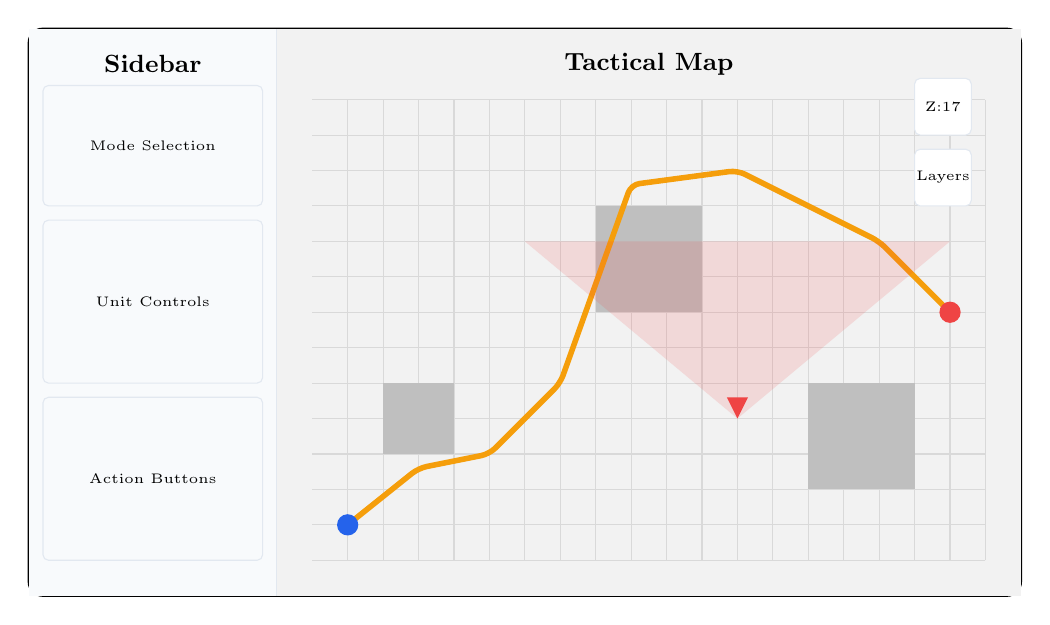
\begin{tikzpicture}[scale=0.9]
    % Main container
    \draw[thick, rounded corners=5pt] (0,0) rectangle (14,8);

    % Sidebar
    \fill[codebg] (0,0) rectangle (3.5,8);
    \draw[codeframe] (3.5,0) -- (3.5,8);
    \node[font=\small\bfseries] at (1.75,7.5) {Sidebar};

    % Sidebar sections
    \draw[codeframe, rounded corners=2pt] (0.2,5.5) rectangle (3.3,7.2);
    \node[font=\tiny] at (1.75,6.35) {Mode Selection};

    \draw[codeframe, rounded corners=2pt] (0.2,3) rectangle (3.3,5.3);
    \node[font=\tiny] at (1.75,4.15) {Unit Controls};

    \draw[codeframe, rounded corners=2pt] (0.2,0.5) rectangle (3.3,2.8);
    \node[font=\tiny] at (1.75,1.65) {Action Buttons};

    % Map area
    \fill[gray!10] (3.5,0) rectangle (14,8);
    \node[font=\small\bfseries] at (8.75,7.5) {Tactical Map};

    % Map grid
    \draw[gray!30, step=0.5] (4,0.5) grid (13.5,7);

    % Buildings on map
    \fill[gray!50] (5,2) rectangle (6,3);
    \fill[gray!50] (8,4) rectangle (9.5,5.5);
    \fill[gray!50] (11,1.5) rectangle (12.5,3);

    % Route example
    \draw[warningamber, line width=2pt, rounded corners=3pt]
        (4.5,1) -- (5.5,1.8) -- (6.5,2) -- (7.5,3) -- (8.5,5.8) -- (10,6) -- (12,5) -- (13,4);

    % Markers
    \fill[primaryblue] (4.5,1) circle (0.15);
    \fill[dangerred] (13,4) circle (0.15);

    % Vision cone
    \fill[dangerred, opacity=0.15] (10,2.5) -- (7,5) -- (13,5) -- cycle;
    \fill[dangerred] (10,2.5) -- (10.15,2.8) -- (9.85,2.8) -- cycle;

    % Zoom indicator
    \draw[codeframe, rounded corners=2pt, fill=white] (12.5,6.5) rectangle (13.3,7.3);
    \node[font=\tiny] at (12.9,6.9) {Z:17};

    % Layer control
    \draw[codeframe, rounded corners=2pt, fill=white] (12.5,5.5) rectangle (13.3,6.3);
    \node[font=\tiny] at (12.9,5.9) {Layers};
\end{tikzpicture}
\caption{GeoRoute Interface Layout}
\label{fig:interface-layout}
\end{figure}

\section{Mode Selection}

GeoRoute provides three distinct operational modes, each designed for a specific use case:

\begin{description}
    \item[Route Mode] is the primary mode for new tactical planning when you need the AI to propose an approach. You define the problem by placing friendly and enemy positions, and the AI generates an optimized tactical route.

    \item[Draw Mode] serves experienced planners who have a specific route in mind and want AI validation and enhancement. Rather than generating routes, the system evaluates your proposed path.

    \item[Simulate Mode] provides the deepest level of analysis by combining geometric modeling with AI vision analysis. This mode is specifically designed for scenarios where enemy positions and orientations are known.
\end{description}

\section{Route Mode (AI Generation)}

The workflow for Route Mode consists of the following steps:

\begin{enumerate}
    \item \textbf{Place Friendly Units}: Click ``Place Soldier'' and click on the map
    \item \textbf{Place Enemy Units}: Click ``Place Enemy'' and click on the map
    \item \textbf{Generate Routes}: Click ``Plan Tactical Attack''
    \item \textbf{Review Results}: Examine the generated routes and tactical report
\end{enumerate}

\begin{notebox}
The system enforces a minimum zoom level of 17 for unit placement. This requirement ensures that positions are specified with sufficient precision for meaningful tactical analysis.
\end{notebox}

\section{Draw Mode (Route Evaluation)}

In Draw Mode, clicking on the map adds waypoints that define your planned movement route:

\begin{enumerate}
    \item Switch to Draw mode using the mode tabs
    \item Click on the map to add waypoints
    \item Configure squad composition (optional)
    \item Click ``Evaluate Route'' for AI analysis
\end{enumerate}

\section{Simulate Mode (Tactical Simulation)}

Simulate Mode provides the most sophisticated analysis:

\begin{enumerate}
    \item \textbf{Place Enemy Units}: Select type (Sniper/Rifleman/Observer) and place on map
    \item \textbf{Set Facing Direction}: Click marker and use ``Rotate +45°'' button
    \item \textbf{Draw Route}: Click waypoints to define movement path
    \item \textbf{Run Simulation}: Click ``Run Simulation'' for cover analysis
\end{enumerate}

\subsection{Understanding Segment Colors}

After simulation analysis, route segments are colored based on cover status:

\begin{itemize}
    \item \textcolor{dangerred}{\textbf{Red}}: Exposed --- no cover blocks line of sight
    \item \textcolor{warningamber}{\textbf{Amber}}: Partial cover --- some concealment exists
    \item \textcolor{secondarygreen}{\textbf{Green}}: Covered --- buildings/walls block enemy view
    \item \textcolor{primaryblue}{\textbf{Blue}}: Clear --- outside all vision cones
\end{itemize}

\section{Report Modal}

The report modal provides comprehensive tactical analysis in a structured format. It appears as an overlay after any analysis operation and contains two primary tabs.

\subsection{Current Analysis Tab}

The Current Analysis tab displays the most recent analysis with the following components:

\begin{description}
    \item[Header] Displays the verdict badge (EXCELLENT, GOOD, ACCEPTABLE, or RISKY), overall rating score, and quick statistics summarizing the analysis.

    \item[Tactical Scores] A radar chart visualization showing the four scoring dimensions: stealth, safety, terrain usage, and flanking advantage. This visual representation allows quick identification of strengths and weaknesses.

    \item[Cover Breakdown] A horizontal bar visualization showing the proportion of route segments that are covered, partially covered, exposed, or clear of enemy observation.

    \item[Flanking Analysis] An approach angle indicator showing the tactical advantage gained from the route's final approach direction relative to enemy facing.

    \item[Annotated Map] The AI-marked satellite image showing the generated or evaluated route with tactical annotations.

    \item[Weak Spots] Specific locations along the route identified as high-risk, with AI-generated recommendations for mitigation.

    \item[Strong Points] Locations where the route effectively exploits terrain features for cover or tactical advantage.

    \item[Recommendations] AI-generated tactical advice for improving the approach or executing the movement.
\end{description}

\subsection{History Tab}

The History tab provides access to all previous analyses from the current session:

\begin{itemize}
    \item Analyses are automatically saved as they are generated
    \item Click any entry to reload that analysis for review
    \item Compare multiple approaches by switching between saved analyses
    \item Clear button removes all saved history
\end{itemize}

\section{Map Controls}

The available map controls are summarized in Table~\ref{tab:map-controls}.

\begin{table}[h]
\centering
\caption{Map Controls}
\label{tab:map-controls}
\begin{tabular}{ll}
\toprule
\textbf{Action} & \textbf{Method} \\
\midrule
Pan & Drag the map \\
Zoom & Scroll wheel or +/- buttons \\
Place unit & Click in placement mode \\
Move unit & Drag the marker \\
Rotate enemy & Click marker $\rightarrow$ Rotate button \\
Remove waypoint & Right-click or sidebar controls \\
Layer switch & Layer control (top-right) \\
\bottomrule
\end{tabular}
\end{table}

% ============================================================================
% CHAPTER 5: SYSTEM ARCHITECTURE
% ============================================================================

\chapter{System Architecture}

Understanding the system architecture enables administrators to troubleshoot issues effectively, developers to extend functionality appropriately, and analysts to appreciate the computational processes underlying their tactical assessments.

\section{High-Level Architecture}

GeoRoute follows a modern microservices-inspired architecture where the frontend and backend operate as independent containerized services communicating through a well-defined API contract. Figure~\ref{fig:high-level-arch} illustrates the major components and their relationships.

\begin{figure}[H]
\centering
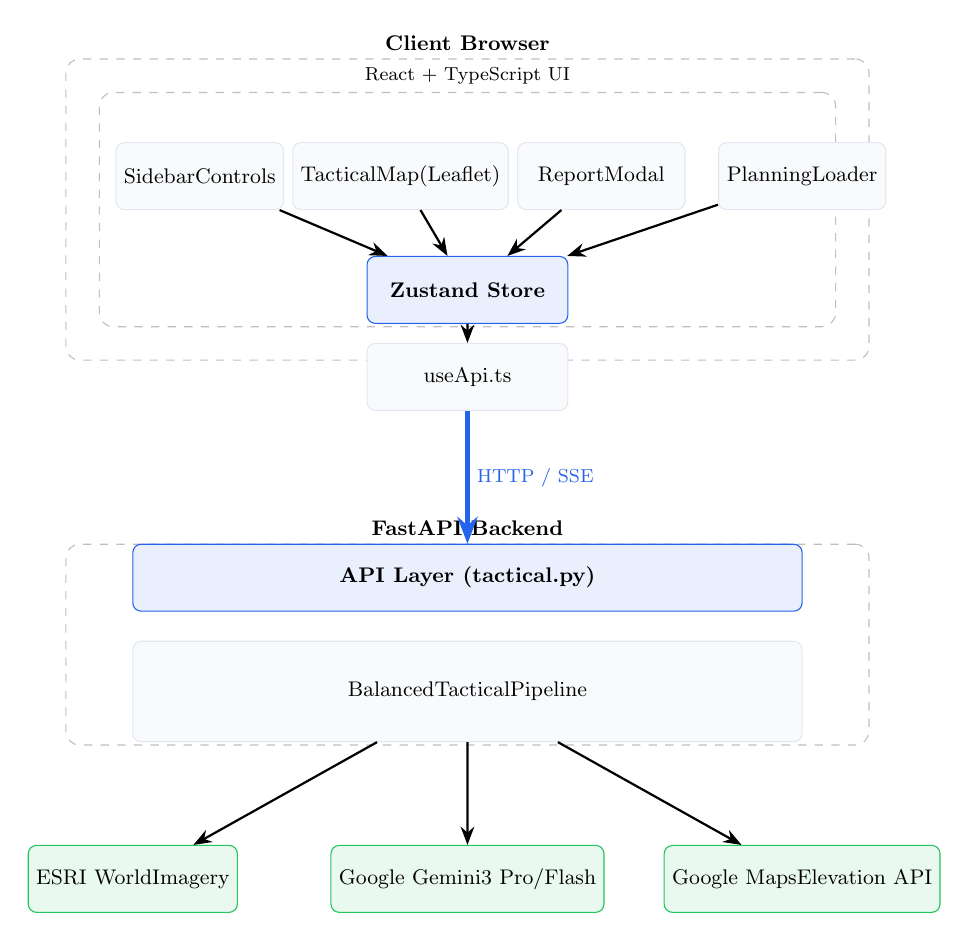
\begin{tikzpicture}[
    node distance=1.5cm,
    scale=0.85,
    transform shape
]
    % Client Browser Container
    \node[container, minimum width=12cm, minimum height=4.5cm, label={[font=\small\bfseries]above:Client Browser}] (browser) at (0,3) {};

    % React UI Container
    \node[container, minimum width=11cm, minimum height=3.5cm, label={[font=\footnotesize]above:React + TypeScript UI}] (reactui) at (0,3) {};

    % UI Components
    \node[component] (sidebar) at (-4,3.5) {Sidebar\\Controls};
    \node[component] (map) at (-1,3.5) {TacticalMap\\(Leaflet)};
    \node[component] (report) at (2,3.5) {Report\\Modal};
    \node[component] (loader) at (5,3.5) {Planning\\Loader};

    % Zustand
    \node[service, minimum width=3cm] (zustand) at (0,1.8) {Zustand Store};

    % useApi
    \node[component, minimum width=3cm] (useapi) at (0,0.5) {useApi.ts};

    % Arrows within browser
    \draw[arrow] (sidebar) -- (zustand);
    \draw[arrow] (map) -- (zustand);
    \draw[arrow] (report) -- (zustand);
    \draw[arrow] (loader) -- (zustand);
    \draw[arrow] (zustand) -- (useapi);

    % Backend Container
    \node[container, minimum width=12cm, minimum height=3cm, label={[font=\small\bfseries]above:FastAPI Backend}] (backend) at (0,-3.5) {};

    % API Layer
    \node[service, minimum width=10cm] (api) at (0,-2.5) {API Layer (tactical.py)};

    % Pipeline
    \node[component, minimum width=10cm, minimum height=1.5cm] (pipeline) at (0,-4.2) {BalancedTacticalPipeline};

    % Connection Browser to Backend
    \draw[arrow, primaryblue, line width=1.5pt] (useapi) -- node[right, font=\footnotesize] {HTTP / SSE} (api);

    % External Services
    \node[external] (esri) at (-5,-7) {ESRI World\\Imagery};
    \node[external] (gemini) at (0,-7) {Google Gemini\\3 Pro/Flash};
    \node[external] (gmaps) at (5,-7) {Google Maps\\Elevation API};

    % Connections to external
    \draw[arrow] (pipeline) -- (esri);
    \draw[arrow] (pipeline) -- (gemini);
    \draw[arrow] (pipeline) -- (gmaps);

\end{tikzpicture}
\caption{High-Level System Architecture}
\label{fig:high-level-arch}
\end{figure}

\section{Request Flow}

The request flow for route generation operations is illustrated in Figure~\ref{fig:request-flow}.

\begin{figure}[H]
\centering
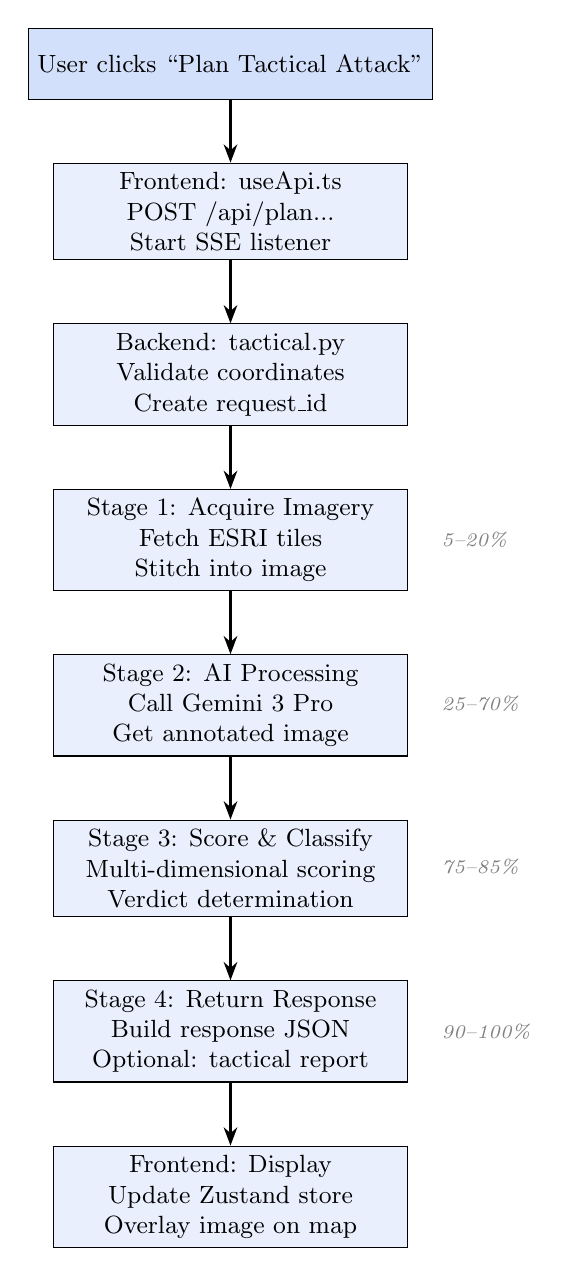
\begin{tikzpicture}[
    node distance=0.8cm,
    process/.style={rectangle, draw, fill=white, minimum width=4.5cm, minimum height=0.9cm, font=\small},
    stage/.style={rectangle, draw, fill=primaryblue!10, minimum width=4.5cm, minimum height=1.2cm, font=\small, align=center},
    progress/.style={font=\scriptsize\itshape, text=gray}
]
    % User action
    \node[process, fill=primaryblue!20] (user) {User clicks ``Plan Tactical Attack''};

    % Frontend
    \node[stage, below=of user] (frontend1) {Frontend: useApi.ts\\POST /api/plan...\\Start SSE listener};

    % Backend
    \node[stage, below=of frontend1] (backend) {Backend: tactical.py\\Validate coordinates\\Create request\_id};

    % Stage 1
    \node[stage, below=of backend] (stage1) {Stage 1: Acquire Imagery\\Fetch ESRI tiles\\Stitch into image};
    \node[progress, right=0.3cm of stage1] {5--20\%};

    % Stage 2
    \node[stage, below=of stage1] (stage2) {Stage 2: AI Processing\\Call Gemini 3 Pro\\Get annotated image};
    \node[progress, right=0.3cm of stage2] {25--70\%};

    % Stage 3
    \node[stage, below=of stage2] (stage3) {Stage 3: Score \& Classify\\Multi-dimensional scoring\\Verdict determination};
    \node[progress, right=0.3cm of stage3] {75--85\%};

    % Stage 4
    \node[stage, below=of stage3] (stage4) {Stage 4: Return Response\\Build response JSON\\Optional: tactical report};
    \node[progress, right=0.3cm of stage4] {90--100\%};

    % Frontend result
    \node[stage, below=of stage4] (frontend2) {Frontend: Display\\Update Zustand store\\Overlay image on map};

    % Arrows
    \draw[arrow] (user) -- (frontend1);
    \draw[arrow] (frontend1) -- (backend);
    \draw[arrow] (backend) -- (stage1);
    \draw[arrow] (stage1) -- (stage2);
    \draw[arrow] (stage2) -- (stage3);
    \draw[arrow] (stage3) -- (stage4);
    \draw[arrow] (stage4) -- (frontend2);

\end{tikzpicture}
\caption{Route Generation Request Flow}
\label{fig:request-flow}
\end{figure}

\section{Data Flow}

The data flow diagram in Figure~\ref{fig:data-flow} illustrates the transformation of data as it moves through the system.

\begin{figure}[H]
\centering
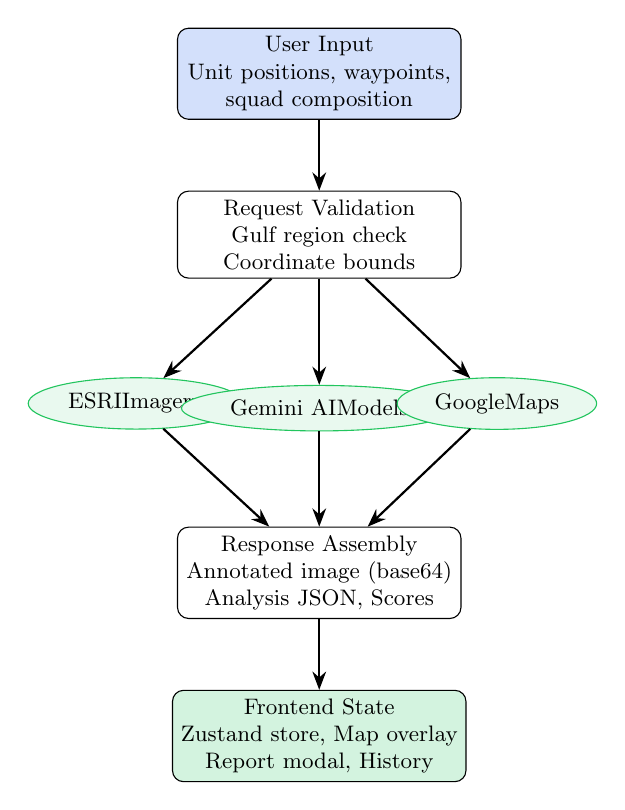
\begin{tikzpicture}[
    node distance=1cm,
    datanode/.style={rectangle, rounded corners, draw, minimum width=4cm, minimum height=1cm, font=\small, align=center},
    extservice/.style={ellipse, draw=secondarygreen, fill=secondarygreen!10, minimum width=2.5cm, font=\small},
    scale=0.9,
    transform shape
]
    % User Input
    \node[datanode, fill=primaryblue!20] (input) {User Input\\Unit positions, waypoints,\\squad composition};

    % Validation
    \node[datanode, below=of input] (validation) {Request Validation\\Gulf region check\\Coordinate bounds};

    % Fan out
    \node[extservice, below left=1.5cm and -0.5cm of validation] (esri) {ESRI\\Imagery};
    \node[extservice, below=1.5cm of validation] (gemini) {Gemini AI\\Models};
    \node[extservice, below right=1.5cm and -0.5cm of validation] (gmaps) {Google\\Maps};

    % Response Assembly
    \node[datanode, below=3.5cm of validation] (assembly) {Response Assembly\\Annotated image (base64)\\Analysis JSON, Scores};

    % Frontend State
    \node[datanode, below=of assembly, fill=secondarygreen!20] (state) {Frontend State\\Zustand store, Map overlay\\Report modal, History};

    % Arrows
    \draw[arrow] (input) -- (validation);
    \draw[arrow] (validation) -- (esri);
    \draw[arrow] (validation) -- (gemini);
    \draw[arrow] (validation) -- (gmaps);
    \draw[arrow] (esri) -- (assembly);
    \draw[arrow] (gemini) -- (assembly);
    \draw[arrow] (gmaps) -- (assembly);
    \draw[arrow] (assembly) -- (state);

\end{tikzpicture}
\caption{Data Flow Through the System}
\label{fig:data-flow}
\end{figure}

A key insight from the data flow is the \textbf{fan-out and fan-in pattern}. A single user request fans out to multiple external services, gathers their results, and fans back into a unified response. This pattern enables parallel service calls where possible, reducing total latency compared to sequential execution.

% ============================================================================
% CHAPTER 6: API REFERENCE
% ============================================================================

\chapter{API Reference}

The GeoRoute API follows REST conventions with JSON request and response bodies. All endpoints are prefixed with \texttt{/api/} to distinguish them from potential future static file serving.

\section{Health Check}

The health check endpoint provides a simple mechanism for monitoring systems to verify that the service is operational.

\begin{itemize}
    \item \textbf{Endpoint:} \texttt{GET /api/health}
    \item \textbf{Response:}
\end{itemize}

\begin{lstlisting}[style=json]
{
  "status": "healthy",
  "timestamp": "2026-02-06T12:00:00Z"
}
\end{lstlisting}

\section{Plan Tactical Attack}

This is the primary endpoint for AI-powered route generation. Due to the complexity of operations involved, this endpoint can take 30 to 90 seconds to complete.

\begin{itemize}
    \item \textbf{Endpoint:} \texttt{POST /api/plan-tactical-attack}
\end{itemize}

\subsection{Request Fields}

\begin{table}[H]
\centering
\begin{tabularx}{\textwidth}{llcX}
\toprule
\textbf{Field} & \textbf{Type} & \textbf{Required} & \textbf{Description} \\
\midrule
request\_id & string & No & Client-provided ID for progress tracking \\
soldiers & array & Yes & List of friendly unit positions \\
enemies & array & Yes & List of enemy unit positions \\
bounds & object & Yes & Map bounds (north, south, east, west) \\
zoom & integer & No & Map zoom level (default: 14) \\
advanced\_analytics & boolean & No & Enable detailed tactical report \\
\bottomrule
\end{tabularx}
\end{table}

\section{Evaluate User Route}

This endpoint evaluates a user-defined route rather than generating new routes.

\begin{itemize}
    \item \textbf{Endpoint:} \texttt{POST /api/evaluate-route}
\end{itemize}

\section{Analyze Tactical Simulation}

The tactical simulation endpoint provides the most sophisticated analysis capability, combining geometric vision cone modeling with AI-based cover assessment.

\begin{itemize}
    \item \textbf{Endpoint:} \texttt{POST /api/analyze-tactical-simulation}
\end{itemize}

\section{Progress Streaming (SSE)}

Long-running operations benefit from real-time progress feedback using Server-Sent Events.

\begin{itemize}
    \item \textbf{Endpoint:} \texttt{GET /api/progress/\{request\_id\}}
\end{itemize}

\subsection{Progress Stages}

\begin{enumerate}
    \item \texttt{imagery} (0--25\%): Fetching satellite imagery
    \item \texttt{routes} or \texttt{analysis} (25--90\%): AI processing
    \item \texttt{report} (90--98\%): Building tactical report
    \item \texttt{complete} (100\%): Done
    \item \texttt{error}: Error occurred
\end{enumerate}

% ============================================================================
% CHAPTER 7: DATA MODELS
% ============================================================================

\chapter{Data Models}

Data models define the structure of information exchanged between system components. In GeoRoute, Pydantic models on the backend and TypeScript interfaces on the frontend ensure type safety and provide self-documenting data contracts.

\section{Unit Models}

\subsection{TacticalUnit}

\begin{lstlisting}[style=python]
class TacticalUnit(BaseModel):
    lat: float          # Latitude position
    lon: float          # Longitude position
    is_friendly: bool   # True for friendly, False for enemy
    unit_id: str | None # Optional unique identifier
\end{lstlisting}

\subsection{SimEnemyUnit}

\begin{lstlisting}[style=python]
class SimEnemyUnit(BaseModel):
    id: str
    type: Literal["sniper", "rifleman", "observer"]
    lat: float
    lng: float
    facing: float  # 0-360 degrees, 0=North
\end{lstlisting}

\section{Analysis Models}

\subsection{SegmentCoverAnalysis}

The SegmentCoverAnalysis model represents the AI's assessment of a single route segment's exposure status.

\begin{lstlisting}[style=python]
class SegmentCoverAnalysis(BaseModel):
    segment_index: int
    in_vision_cone: bool
    cover_status: Literal["exposed", "covered", "partial", "clear"]
    cover_type: str | None  # "building", "vegetation", "terrain"
    exposure_percentage: float  # 0-100
    blocking_feature: str | None
    enemy_id: str | None
    explanation: str
\end{lstlisting}

\subsection{TacticalScores}

\begin{lstlisting}[style=python]
class TacticalScores(BaseModel):
    stealth: float       # 0-100: How hidden is the approach
    safety: float        # 0-100: Survival probability
    terrain_usage: float # 0-100: How well route uses cover
    flanking: float      # 0-100: Approach angle advantage
    overall: float       # 0-100: Weighted composite
\end{lstlisting}

\subsection{FlankingAnalysis}

\begin{lstlisting}[style=python]
class FlankingAnalysis(BaseModel):
    is_flanking: bool      # Approaching from enemy blind spot?
    approach_angle: float  # 0-360 degrees from enemy facing
    bonus_awarded: float   # 0-3 rating points bonus
    description: str
\end{lstlisting}

\subsection{CoverBreakdown}

\begin{lstlisting}[style=python]
class CoverBreakdown(BaseModel):
    total_segments: int
    exposed_count: int
    covered_count: int
    partial_count: int
    clear_count: int
    overall_cover_percentage: float  # 0-100
    cover_types_used: list[str]
\end{lstlisting}

% ============================================================================
% CHAPTER 8: AI PROMPTS
% ============================================================================

\chapter{AI Prompts \& Customization}

The quality of GeoRoute's tactical analysis depends heavily on the prompts provided to the Gemini AI models. These prompts are essentially detailed instructions that tell the AI what to look for in satellite imagery, how to evaluate tactical situations, and what format to use for responses.

\section{Prompt Location}

All AI prompts reside in the \texttt{georoute/config.yaml} file, which is read fresh for each API request. This means prompt changes take effect immediately without restarting the backend service.

\begin{table}[H]
\centering
\caption{AI Prompts in Configuration}
\begin{tabular}{ll}
\toprule
\textbf{Prompt} & \textbf{Purpose} \\
\midrule
\texttt{route\_prompt} & Instructions for Gemini to draw routes \\
\texttt{analysis\_prompt} & Advanced tactical analysis \\
\texttt{route\_evaluation\_prompt} & User-drawn route analysis \\
\texttt{tactical\_simulation\_prompt} & Vision cone + cover analysis \\
\bottomrule
\end{tabular}
\end{table}

\section{Route Drawing Prompt}

The route drawing prompt instructs Gemini 3 Pro to analyze a satellite image with marked start and end positions, then draw a tactical infantry movement route directly on the image. Key elements include:

\begin{itemize}
    \item Single route generation
    \item Line color (cyan)
    \item Drawing style (thin, smooth curves)
    \item Obstacle avoidance rules (follow streets, avoid buildings)
\end{itemize}

\section{Tactical Simulation Prompt}

The tactical simulation prompt guides the AI through multi-step analysis:

\begin{enumerate}
    \item Understand the tactical scenario from the annotated satellite image
    \item Identify enemy positions and facing directions from vision cones
    \item Analyze each route segment for cover status
    \item Apply scoring rules for exposure and flanking
    \item Output structured JSON response
\end{enumerate}

\begin{warningbox}
The JSON output format must remain consistent with backend Pydantic models. Changing field names, types, or structure in the prompt without corresponding backend changes will cause parsing failures.
\end{warningbox}

\section{Modifying Prompts}

The recommended workflow for prompt modification:

\begin{enumerate}
    \item Edit \texttt{georoute/config.yaml} with proposed changes
    \item Save the file (changes take effect immediately)
    \item Run several test analyses with known scenarios
    \item Compare AI output to expected results
    \item Iterate until output is satisfactory
    \item Monitor backend logs for parsing errors
\end{enumerate}

% ============================================================================
% CHAPTER 9: FRONTEND ARCHITECTURE
% ============================================================================

\chapter{Frontend Architecture}

The GeoRoute frontend is built with React and TypeScript, providing a type-safe, component-based architecture that facilitates maintenance and extension.

\section{Component Hierarchy}

\begin{lstlisting}[basicstyle=\ttfamily\small,frame=none,numbers=none]
App.tsx
 |-- Index.tsx (Main page)
     |-- Sidebar.tsx
     |   |-- UnitPlacement.tsx
     |   |-- ActionButtons.tsx
     |   |-- SimulationControls.tsx
     |   |-- RouteDrawingControls.tsx
     |   |-- UnitCompositionPanel.tsx
     |
     |-- TacticalMap.tsx
     |   |-- ZoomIndicator.tsx
     |
     |-- TacticalReportModal.tsx
     |-- PlanningLoader.tsx
\end{lstlisting}

\section{State Management (Zustand)}

Zustand provides global state management with a minimal API. The store is defined as a single hook (\texttt{useMission}) that components call to access and modify state. Unlike Redux, Zustand requires minimal boilerplate while providing the same global state capabilities. Components subscribe to specific slices of state, preventing unnecessary re-renders when unrelated state changes.

\section{API Layer (useApi.ts)}

The API layer abstracts HTTP communication with the backend, providing consistent error handling and progress tracking. All API calls flow through utility functions that handle JSON serialization, error extraction, and response parsing. This centralization ensures that error handling logic is consistent throughout the application and simplifies adding new API calls.

\subsection{HTTP Request Handling}

\begin{lstlisting}[style=typescript]
async function fetchWithError(url: string, options: RequestInit) {
  const response = await fetch(url, options);
  if (!response.ok) {
    const error = await response.json().catch(() => ({}));
    throw new Error(error.detail || error.message || 'Request failed');
  }
  return response;
}
\end{lstlisting}

The error handling logic specifically extracts the \texttt{detail} field from error responses, which is where FastAPI places structured error messages. This allows the backend to provide meaningful, user-friendly error messages that the frontend displays without modification.

\subsection{SSE Progress Streaming}

Server-Sent Events provide real-time progress updates during long-running AI operations:

\begin{lstlisting}[style=typescript]
function subscribeToProgress(requestId: string, onProgress: Function) {
  const eventSource = new EventSource(`${API_URL}/api/progress/${requestId}`);
  eventSource.onmessage = (event) => {
    const data = JSON.parse(event.data);
    onProgress(data);
  };
  return () => eventSource.close();
}
\end{lstlisting}

The SSE connection is established before the main API call, ensuring progress updates are received from the moment processing begins. The returned cleanup function is called when the component unmounts or when the operation completes.

\section{Map Layer (TacticalMap.tsx)}

The map uses a layered architecture as shown in Table~\ref{tab:map-layers}.

\begin{table}[H]
\centering
\caption{Map Layers}
\label{tab:map-layers}
\begin{tabular}{ll}
\toprule
\textbf{Layer} & \textbf{Purpose} \\
\midrule
\texttt{tileLayers.satellite} & ESRI World Imagery base \\
\texttt{unitMarkers} & Soldier/enemy markers \\
\texttt{simEnemyMarkers} & Simulation enemy markers \\
\texttt{simEnemyVisionCones} & Red vision cone polygons \\
\texttt{drawnRoutePolyline} & User-drawn route line \\
\texttt{planOverlays} & Gemini-generated route images \\
\bottomrule
\end{tabular}
\end{table}

% ============================================================================
% CHAPTER 10: BACKEND ARCHITECTURE
% ============================================================================

\chapter{Backend Architecture}

The GeoRoute backend is built with FastAPI, a modern Python web framework that provides automatic API documentation, request validation through Pydantic models, and native support for asynchronous operations.

\section{Module Structure}

\begin{lstlisting}[basicstyle=\ttfamily\small,frame=none,numbers=none]
georoute/
|-- main.py                 # FastAPI app entry point
|-- config.py               # Configuration loading
|-- config.yaml             # All settings and prompts
|-- api/
|   |-- routes.py           # Health check
|   |-- tactical.py         # Main API endpoints
|-- clients/
|   |-- esri_imagery.py     # Satellite tile fetching
|   |-- gemini_tactical.py  # Gemini AI client
|   |-- google_maps.py      # Elevation API client
|-- models/
|   |-- tactical.py         # Pydantic data models
|-- processing/
|   |-- balanced_tactical_pipeline.py
|   |-- gemini_image_route_generator.py
|-- utils/
    |-- geo_validator.py    # Gulf region validation
\end{lstlisting}

\section{Pipeline Classes}

\subsection{BalancedTacticalPipeline}

The BalancedTacticalPipeline class is the primary orchestration component. It is instantiated with configuration and client dependencies, then exposes methods for each type of analysis.

\subsection{GeminiImageRouteGenerator}

This class encapsulates all interactions with Google's Gemini AI models, handling both AI Studio and Vertex AI authentication paths.

\section{Error Handling}

Error handling serves two purposes: providing useful feedback to users and protecting internal system details from exposure.

\begin{lstlisting}[style=python]
def _sanitize_error(e: Exception) -> tuple[str, int]:
    """Convert exceptions to user-friendly messages."""
    error_str = str(e).lower()

    if "resource_exhausted" in error_str:
        return "Rate limit exceeded. Please wait.", 429

    if "permission_denied" in error_str:
        return "Authentication failed. Check API key.", 401

    return "An error occurred during analysis.", 500
\end{lstlisting}

\section{NGINX Reverse Proxy}

Version 2.0 introduces NGINX as the default entry point for all traffic. This production-grade reverse proxy provides several critical capabilities that improve security, performance, and scalability.

\subsection{Why NGINX?}

Direct exposure of application services to the internet introduces unnecessary risk. NGINX serves as a protective layer that:

\begin{itemize}
    \item \textbf{Terminates external connections} before they reach application code
    \item \textbf{Enforces rate limits} to prevent abuse and denial-of-service attempts
    \item \textbf{Compresses responses} to reduce bandwidth usage
    \item \textbf{Adds security headers} to protect against common web vulnerabilities
    \item \textbf{Load balances} across multiple backend instances
\end{itemize}

\subsection{Configuration}

The NGINX configuration resides in \texttt{nginx/nginx.conf}. Key settings include:

\textbf{Rate Limiting:}
\begin{lstlisting}[style=bash]
limit_req_zone $binary_remote_addr zone=api_limit:10m rate=10r/s;
\end{lstlisting}

API endpoints are limited to 10 requests per second per IP address, with a burst allowance of 20 requests. This prevents individual users from overwhelming the AI processing pipeline.

\textbf{Load Balancing with Sticky Sessions:}
\begin{lstlisting}[style=bash]
upstream backend {
    ip_hash;  # Sticky sessions - same client always goes to same backend
    server georoute-backend:9001;
    keepalive 32;
}
\end{lstlisting}

When multiple backend replicas are running, NGINX uses IP hash for sticky sessions. This ensures the same client always routes to the same backend, which is required for SSE progress updates to work correctly (progress state is stored in-memory per backend instance).

\textbf{AI Operation Timeouts:}
\begin{lstlisting}[style=bash]
proxy_read_timeout 180s;
proxy_connect_timeout 60s;
\end{lstlisting}

AI operations can take up to 3 minutes. Standard timeout values would terminate these requests prematurely.

\textbf{SSE Support:}
\begin{lstlisting}[style=bash]
proxy_buffering off;
proxy_cache off;
chunked_transfer_encoding on;
\end{lstlisting}

Server-Sent Events require special handling to maintain persistent connections for progress streaming.

\subsection{Scaling Backend Replicas}

To handle more concurrent users, scale the backend service:

\begin{lstlisting}[style=bash]
# Scale to 3 replicas
docker compose up -d --scale georoute-backend=3

# Scale back to 1
docker compose up -d --scale georoute-backend=1
\end{lstlisting}

NGINX automatically discovers new replicas through Docker's DNS resolution and distributes load accordingly.

\textbf{When to scale:}
\begin{itemize}
    \item Multiple analysts working simultaneously
    \item AI operations causing request queuing
    \item Response times increasing under load
\end{itemize}

\textbf{Scaling limits:}
\begin{itemize}
    \item Gemini API rate limits remain the true bottleneck ($\sim$60 req/min)
    \item Each replica consumes $\sim$500MB RAM
    \item More than 5 replicas rarely provides benefit
\end{itemize}

% ============================================================================
% CHAPTER 11: TROUBLESHOOTING
% ============================================================================

\chapter{Troubleshooting}

This chapter provides guidance for diagnosing and resolving common issues that may arise during GeoRoute operation.

\section{Common Issues}

\subsection{``Outside Gulf Region'' Error}

\begin{description}
    \item[Cause:] Coordinates are outside the GCC bounding box.
    \item[Solution:] Ensure all coordinates are within:
    \begin{itemize}
        \item Latitude: 12°N to 32°N
        \item Longitude: 34°E to 60°E
    \end{itemize}
\end{description}

\subsection{``Zoom In Required'' Popup}

\begin{description}
    \item[Cause:] Map zoom level is below 17.
    \item[Solution:] Zoom in to level 17 or higher before placing units.
\end{description}

\subsection{No Routes Generated}

\begin{description}
    \item[Causes:] Invalid Gemini API key, rate limit exceeded, or model unavailable.
    \item[Solutions:]
    \begin{itemize}
        \item Check API key in \texttt{.env}
        \item Wait 1--2 minutes and retry
        \item Check \texttt{docker compose logs georoute-backend}
    \end{itemize}
\end{description}

\section{Log Analysis}

\begin{lstlisting}[style=bash]
# View all logs
docker compose logs -f

# Backend only
docker compose logs -f georoute-backend

# Search for errors
docker compose logs | grep -i error
\end{lstlisting}

\section{Health Checks}

\begin{lstlisting}[style=bash]
# Check backend health
curl http://localhost:8001/api/health

# Check container status
docker compose ps

# Check resource usage
docker stats
\end{lstlisting}

% ============================================================================
% CHAPTER 12: EXTENDING THE SYSTEM
% ============================================================================

\chapter{Extending the System}

GeoRoute is designed with extensibility in mind. The modular architecture, externalized configuration, and clear separation between layers facilitate adding new capabilities.

\section{Adding New Enemy Types}

\begin{enumerate}
    \item \textbf{Backend} (\texttt{models/tactical.py}): Add to enum
    \item \textbf{Backend} (\texttt{balanced\_tactical\_pipeline.py}): Add vision specs
    \item \textbf{Frontend} (\texttt{useMission.ts}): Add to \texttt{ENEMY\_VISION\_SPECS}
    \item \textbf{Frontend} (\texttt{TacticalMap.tsx}): Add icon
\end{enumerate}

\section{Adding New Scoring Metrics}

\begin{enumerate}
    \item Update \texttt{TacticalScores} model in backend
    \item Modify \texttt{tactical\_simulation\_prompt} to calculate metric
    \item Update TypeScript interfaces in frontend
    \item Update visualization components
\end{enumerate}

\section{Adding New Analysis Modes}

New analysis modes enable entirely new types of tactical assessment. For example, you might add a ``defensive position evaluation'' mode for assessing fortification locations, or a ``convoy route planning'' mode optimized for vehicle movement. Adding a mode is the most substantial extension, requiring new endpoints, processing logic, data models, and UI components.

The existing modes provide templates for implementation. Follow their patterns for request validation, progress reporting, and response formatting to maintain consistency. Consider how the new mode relates to existing modes and whether it should share UI space (as route and draw modes do in the sidebar) or require new interface elements.

Implementation steps:
\begin{enumerate}
    \item Create new endpoint in \texttt{tactical.py}
    \item Add pipeline method in \texttt{balanced\_tactical\_pipeline.py}
    \item Add request/response models in \texttt{models/tactical.py}
    \item Create frontend components for the new mode
    \item Add state management in \texttt{useMission.ts}
    \item Connect to sidebar controls
\end{enumerate}

\section{Changing AI Models}

Model selection is configuration-driven. Edit \texttt{georoute/config.yaml}:

\begin{lstlisting}[style=yaml]
gemini:
  image_model: "gemini-3-pro-image-preview"
  text_model: "gemini-2.5-flash"
  analysis_model: "gemini-3-flash-preview"
\end{lstlisting}

No code changes required --- models are loaded from config.

% ============================================================================
% APPENDICES
% ============================================================================

\appendix

\chapter{Glossary}

\begin{description}
    \item[Cover] Physical obstruction that blocks line of sight
    \item[Concealment] Visual obstruction that hides but doesn't block fire
    \item[Vision Cone] Triangle representing enemy field of view
    \item[Flanking] Approaching from enemy's blind spot ($>$90° from facing)
    \item[LOS] Line of Sight
    \item[SSE] Server-Sent Events (real-time progress streaming)
    \item[GCC] Gulf Cooperation Council (regional restriction)
    \item[NGINX] High-performance web server used as reverse proxy
    \item[Sticky Sessions] Load balancing technique that routes same client to same server
    \item[Vertex AI] Google Cloud's managed AI platform for production deployments
\end{description}

\chapter{Keyboard Shortcuts}

The current version of GeoRoute relies on mouse-based interactions through the map interface. Keyboard shortcuts have not been implemented in this release but may be added in future versions based on user feedback and operational requirements.

Priority shortcut candidates for future implementation:
\begin{itemize}
    \item Mode switching (Route/Draw/Simulate)
    \item Unit type selection
    \item Report navigation
    \item Map zoom controls
    \item Quick actions (clear, undo)
\end{itemize}

\chapter{Version History}

\begin{table}[H]
\centering
\begin{tabularx}{\textwidth}{llX}
\toprule
\textbf{Version} & \textbf{Date} & \textbf{Changes} \\
\midrule
2.0 & Feb 2026 & Production infrastructure: NGINX reverse proxy with rate limiting and load balancing, Vertex AI as recommended backend, unified docker-compose.yml, backend scaling support with sticky sessions, security headers, SSE proxy support, error sanitization. \\
\midrule
1.0 & Feb 2026 & Initial release with AI-powered route generation, user route evaluation, and tactical simulation with vision cone modeling. Includes Vertex AI support and comprehensive reporting. \\
\bottomrule
\end{tabularx}
\end{table}

% ============================================================================
% CLOSING
% ============================================================================

\chapter*{Closing Notes}
\addcontentsline{toc}{chapter}{Closing Notes}

GeoRoute represents the application of cutting-edge AI technology to the longstanding challenge of tactical route planning. While the system provides powerful analytical capabilities, it is designed to augment rather than replace human judgment. The verdicts, scores, and recommendations should be considered as inputs to decision-making, not as directives.

Feedback from operational use is essential for continued improvement. As you work with the system, note any scenarios where the analysis seems inconsistent or where additional capabilities would be valuable. This feedback informs prompt refinement, feature prioritization, and overall system evolution.

\vspace{1cm}
\noindent\textit{This manual is maintained alongside the GeoRoute codebase. For questions, issues, or contributions, see the project repository.}

\end{document}
